\documentclass{standalone}
%\documentclass[11pt,hyperref={colorlinks=false,runcolor=blue}]{beamer}
\usepackage{DejaVuSans} % Define font
\renewcommand*\familydefault{\sfdefault} %% Only if the base font of the document is to be sans serif
\usepackage[T1]{fontenc}
%\usepackage{lmodern}
\usepackage{tikz}
\usetikzlibrary{backgrounds,fit,calc,shadows,chains,ocgx,shapes.geometric,arrows.meta,positioning}
%\usepackage{microtype}
\usepackage{url}
%\usepackage{fancyvrb}
%\usepackage{listings}
\usepackage{pgfplots}

\usetikzlibrary{decorations.text} % for text along curved paths


\definecolor{mybrown}{RGB}{200,92,35}
\definecolor{myolive}{RGB}{200,175,35}
\definecolor{myleaf}{RGB}{143,200,35}
\definecolor{mygreen}{RGB}{61,200,35}

\definecolor{mypurple}{RGB}{200,35,162}
\definecolor{mypink}{RGB}{200,35,79}
\definecolor{myred}{RGB}{200,73,35}
\definecolor{myorange}{RGB}{200,155,35}


% USE readarray  TO GET THE DATA INTO A \def
\usepackage{readarray}
\readarraysepchar{;}

\usepackage{etoolbox}

% for too large figure margins because of bounding boxes around the tikz figure
\usepackage{adjustbox}

\begin{document}



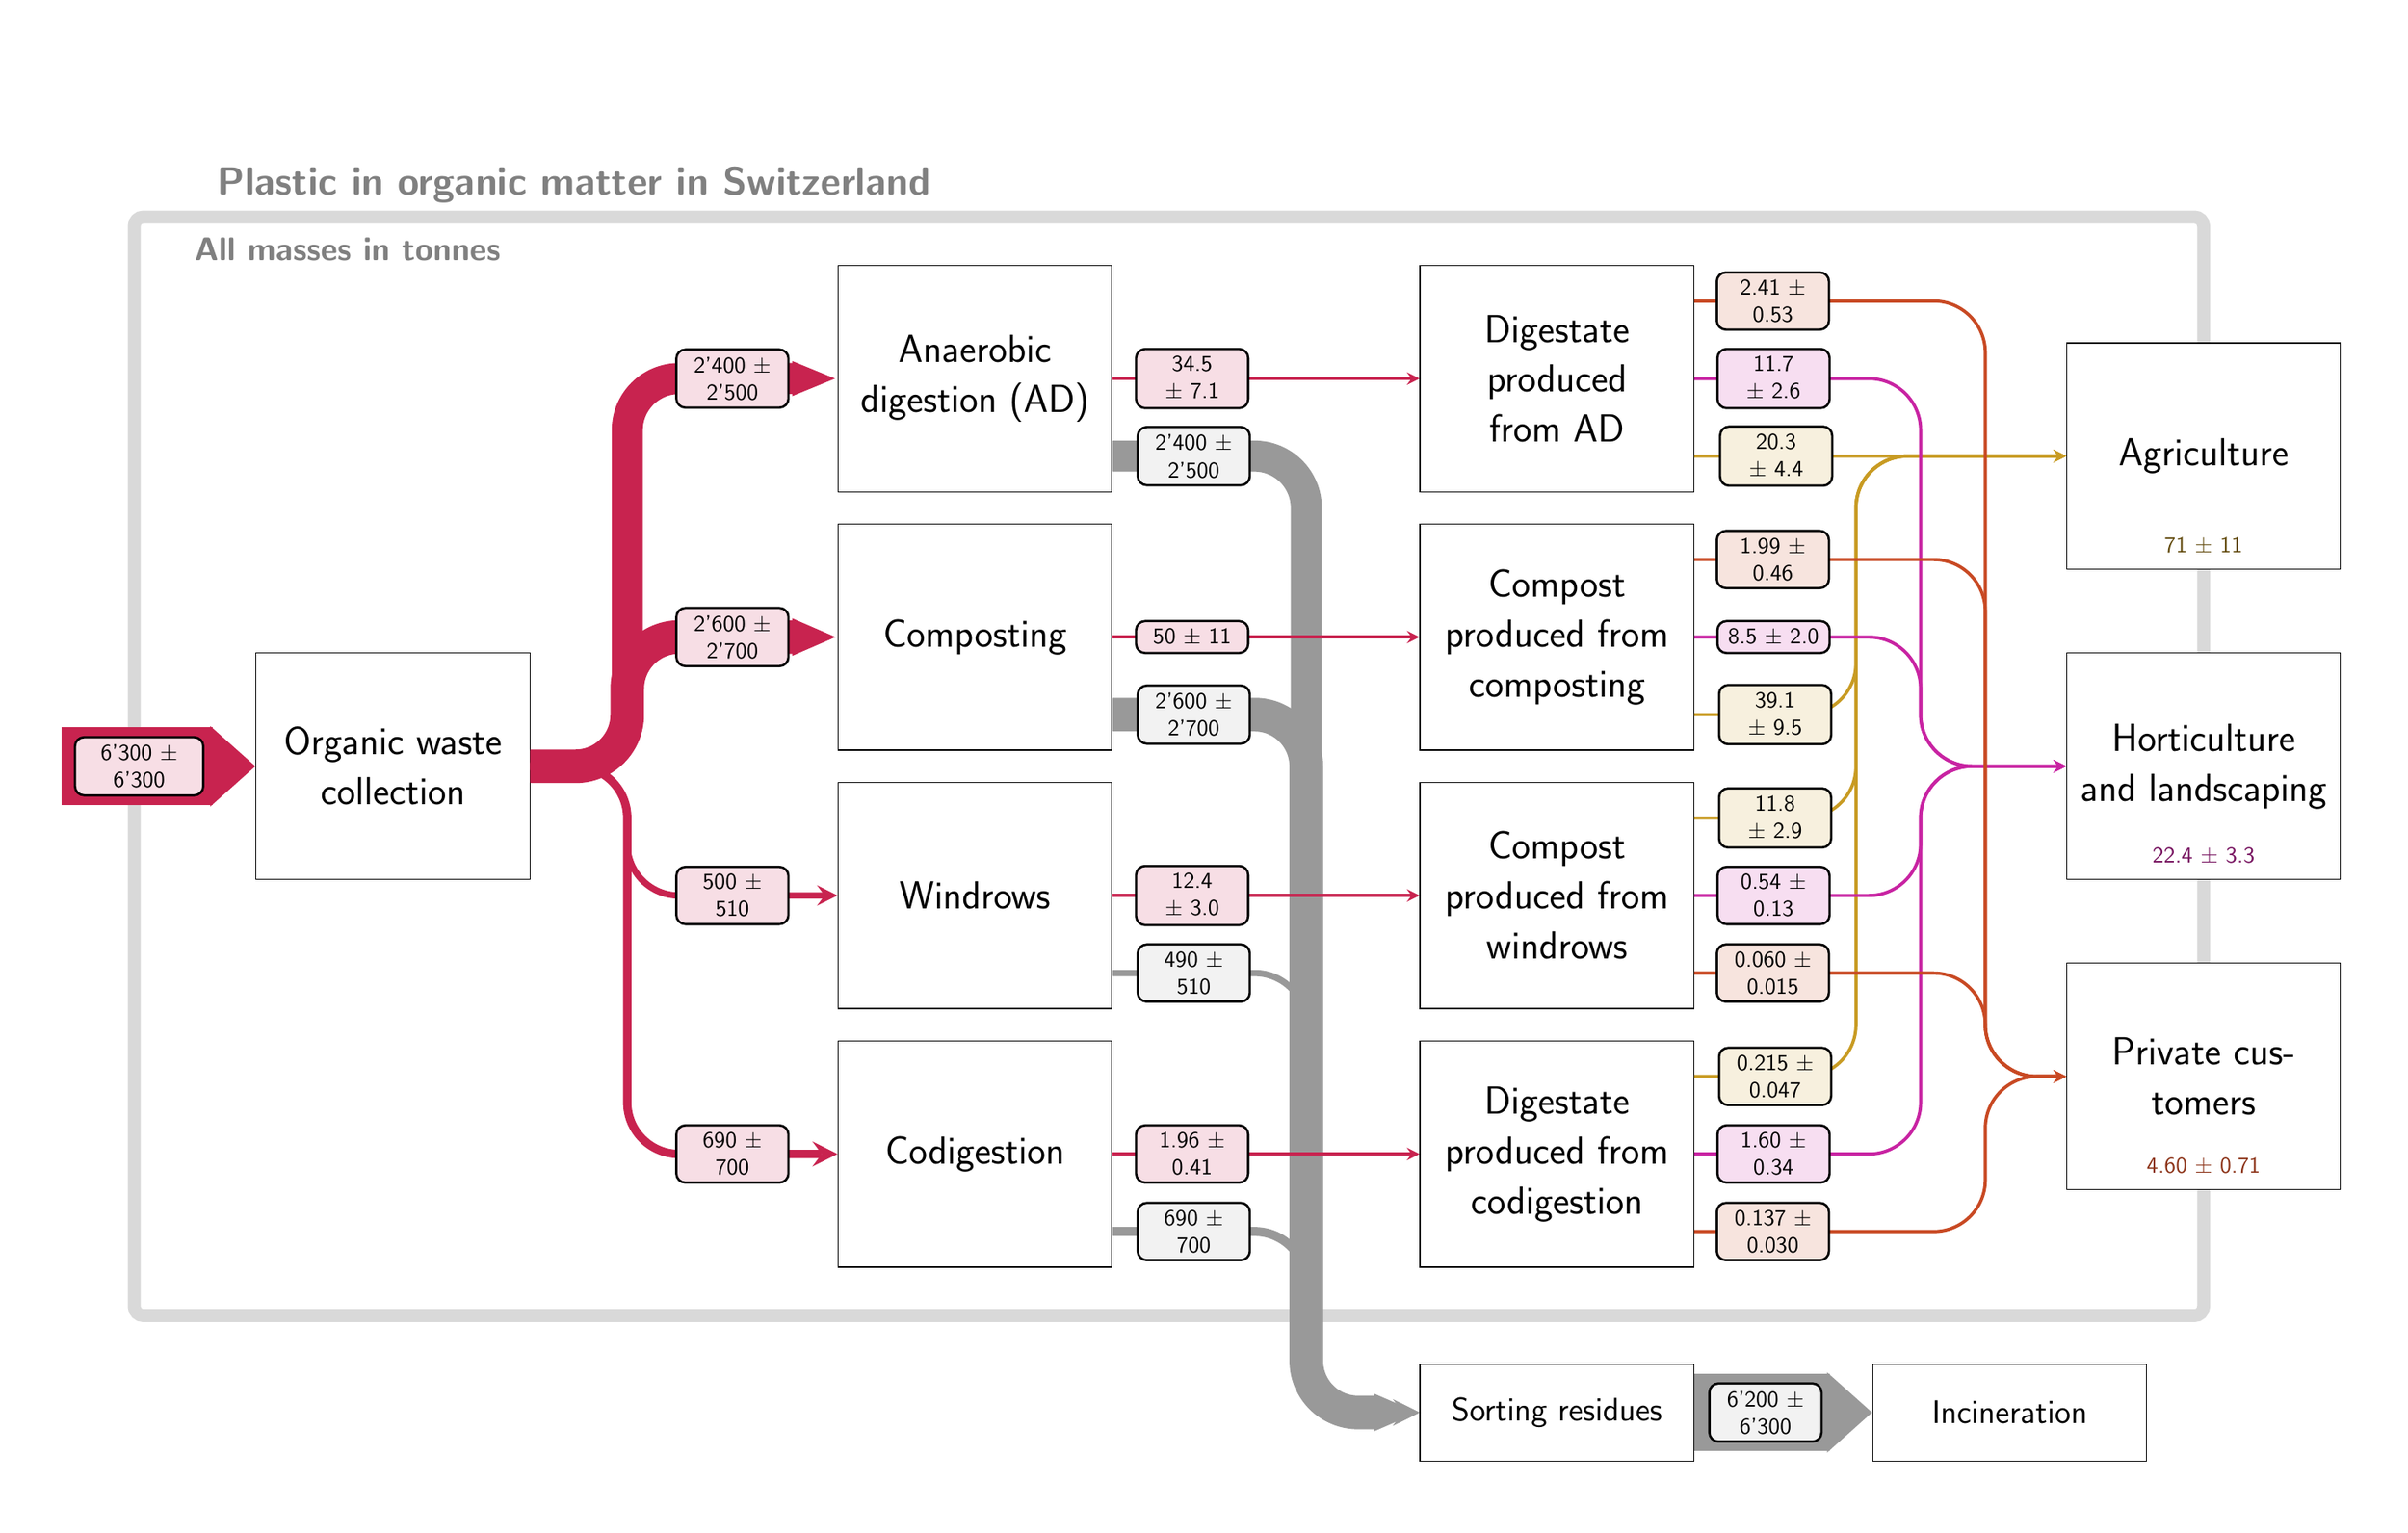
\begin{tikzpicture}[
		comp/.style ={rectangle,fill = white, draw=black, text width = 4 cm, text centered, minimum height=3.5cm, font=\LARGE},
		compMP/.style ={rectangle,fill = black!10!red!10, draw=black, text width = 3 cm, text centered, minimum height=0.8cm, yshift=-1cm},
		flow/.style  ={-stealth, line width = 4, rounded corners=8mm, draw=mypink},
		flow1/.style  ={flow, draw = myorange},
		flow2/.style  ={flow, draw = mypurple},
		flow3/.style  ={flow, draw = myred},
		flow4/.style  ={flow, draw = black!40},
		flow5/.style  ={flow, draw = black!20},
		labs/.style   ={rectangle, rounded corners, fill = mypink!15, draw=black ,text centered, line width = 1, text width = 1.5 cm},
		labs1/.style  ={labs, fill = myorange!15},
		labs2/.style  ={labs, fill = mypurple!15},
		labs3/.style  ={labs, fill = myred!15},
		labs4/.style  ={labs, fill = black!5},
		labs5/.style  ={labs, fill = white}]

% figure size
\draw[draw = white] (-5,13.5) rectangle ++(35.8,-23) {};

% system boundary
\draw[draw = black!15, line width = 2 mm, rounded corners] (-4,-6.5) rectangle ++(32,17) {};
\node[font=\LARGE,text=black!50](title) at (2.8,11){\textbf{\textit{Plastic in organic matter in Switzerland}}};
\node[font=\Large,text=black!50](title) at (-.7,10){\textbf{\textit{All masses in tonnes}}};


%%%%%%%%%%%%%%%%%%%%%%%%%%%%%%%%%%%%%%%%%%%%%%%%%%%%%%%%%%%%%%%%%%
%%%%%%%%%%%%%%%%% COMPARTMENTS %%%%%%%%%%%%%%%%%%%%%%%%%%%%%%%%%%%
%%%%%%%%%%%%%%%%%%%%%%%%%%%%%%%%%%%%%%%%%%%%%%%%%%%%%%%%%%%%%%%%%%


\node[comp] (coll) at (0,2)   {Organic waste collection} ;

\node[comp] (ad)   at (9,8)  {Anaerobic digestion (AD)} ;
\node[comp] (comp) at (9,4)  {Composting} ;
\node[comp] (win)  at (9,0)  {Windrows} ;
\node[comp] (cod)  at (9,-4) {Codigestion} ;

%\node[comp, minimum height=1.5cm, font=\Large] (loss)  at (9,-8) {Losses during transfer} ;

\node[comp] (ad2)   at (18,8)  {Digestate produced from AD} ;
\node[comp] (comp2) at (18,4)  {Compost produced from composting} ;
\node[comp] (win2)  at (18,0)  {Compost produced from windrows} ;
\node[comp] (cod2)  at (18,-4) {Digestate produced from codigestion} ;

\node[comp, minimum height=1.5cm, font=\Large] (res)  at (18,-8) {Sorting residues} ;
\node[comp, minimum height=1.5cm, font=\Large] (inc)  at (25,-8) {Incineration} ;
%\node[comp, minimum height=1.5cm, font=\Large] (oth)  at (18,12) {Other products} ;

\node[comp] (agri)  at (28,6.8)  {Agriculture} ;
\node[comp] (horti) at (28,2)  {Horticulture and landscaping} ;
\node[comp] (priv)  at (28,-2.8) {Private customers} ;

\node[text=myorange!50!black] (text) at ([shift={(0,-1.4)}]agri)  {71 $\pm$ 11};
\node[text=mypurple!60!black] (text) at ([shift={(0,-1.4)}]horti) {22.4 $\pm$ 3.3};
\node[text=myred!70!black] (text) at ([shift={(0,-1.4)}]priv)  {4.60 $\pm$ 0.71};


%%%%%%%%%%%%%%%%%%%%%%%%%%%%%%%%%%%%%%%%%%%%%%%%%%%%%%%%%%%%%%%%%%
%%%%%%%%%%%%%%%%% PATHWAYS %%%%%%%%%%%%%%%%%%%%%%%%%%%%%%%%%%%%%%%
%%%%%%%%%%%%%%%%%%%%%%%%%%%%%%%%%%%%%%%%%%%%%%%%%%%%%%%%%%%%%%%%%%

% INFLOW

\draw[flow, line width = 1.2cm,-{Triangle[length=.7cm,width=1.2cm]}]
	([shift={(-3,0)}]coll.west) -- (coll.west)
	node[labs, pos = .4, text width = 1.75 cm] {6'300 $\pm$ 6'300};

\draw[flow, line width = .48cm,-{Triangle[length=.7cm,width=.48cm]}]
	(coll.east) -- ++(1.5,0) |- (ad.west)
	node[labs, pos = .75] {2'400 $\pm$ 2'500};
\draw[flow, line width = .52cm, -{Triangle[length=.7cm,width=.52cm]}]
	(coll.east) -- ++(1.5,0) |- (comp.west)
	node[labs, pos = .75] {2'600 $\pm$ 2'700};
\draw[flow, line width = .1cm]
	(coll.east) -- ++(1.5,0) |- (win.west)
	node[labs, pos = .75] {500 $\pm$ 510};
\draw[flow, line width = .13cm]
	(coll.east) -- ++(1.5,0) |- (cod.west)
	node[labs, pos = .75] {690 $\pm$ 700};
%\draw[flow, line width = .05cm]
%	(coll.east) -- ++(1.5,0) |- (loss.west)
%	node[labs, pos = .75] {19 $\pm$ 19};

%\draw[flow5, line width = .39cm,-{Triangle[length=.7cm,width=.39cm]}] 
%	([shift={(0,1.2)}]ad.east)   -- ++(3.5,0)
%	node[labs5, pos = .35] {}
%	|- (oth.west);
%\draw[flow5, line width = .25cm] ([shift={(0,1.2)}]comp.east) -- ++(3.5,0)
%	node[labs5, pos = .35] {}
%	 |- (oth.west);
%\draw[flow5, line width = .1cm]
%	([shift={(0,1.2)}]win.east)  -- ++(3.5,0)
%	node[labs5, pos = .35] {490 $\pm$ 510}
%	 |- (oth.west);
%\draw[flow5, line width = .13cm]
%	([shift={(0,1.2)}]cod.east)  -- ++(3.5,0)
%	node[labs5, pos = .35] {690 $\pm$ 700}
%	|- (oth.west);

\draw[flow4, line width = .48cm,-{Triangle[length=.7cm,width=.48cm]}]
	([shift={(0,-1.2)}]ad.east)   -- ++(3,0)
	node[labs4, pos = .42] {2'400 $\pm$ 2'500}
	|- (res.west);
\draw[flow4, line width = .52cm,-{Triangle[length=.7cm,width=.52cm]}]
	([shift={(0,-1.2)}]comp.east) -- ++(3,0)
	node[labs4, pos = .42] {2'600 $\pm$ 2'700}
	|- (res.west);
\draw[flow4, line width = .1cm] ([shift={(0,-1.2)}]win.east)  -- ++(3,0)
	node[labs4, pos = .42] {490 $\pm$ 510}
	|- (res.west);
\draw[flow4, line width = .14cm] ([shift={(0,-1.2)}]cod.east)  -- ++(3,0)
	node[labs4, pos = .42] {690 $\pm$ 700}
	|- (res.west);

\draw[flow4, line width = 1.2cm,-{Triangle[length=.7cm,width=1.2cm]}]
	(res.east) -- (inc.west)
	node[labs4, pos = .4] {6'200 $\pm$ 6'300};

\draw[flow, line width = .05cm] (ad)   -- (ad2)
	node[labs, pos = .26] {34.5 $\pm$ 7.1};
\draw[flow, line width = .05cm] (comp) -- (comp2)
	node[labs, pos = .26] {50 $\pm$ 11};
\draw[flow, line width = .05cm] (win)  -- (win2)
	node[labs, pos = .26] {12.4 $\pm$ 3.0};
\draw[flow, line width = .05cm] (cod)  -- (cod2)
	node[labs, pos = .26] {1.96 $\pm$ 0.41};

\draw[flow1, line width = .05cm]
	([shift={(0,-1.2)}]ad2.east) -- (agri.west)
	node[labs1, pos = .22] {20.3 $\pm$ 4.4};
\draw[flow1, line width = .05cm]
	([shift={(0,-1.2)}]comp2.east) -- ++(2.5,0)
	node[labs1, pos = .5] {39.1 $\pm$ 9.5}
	|- (agri.west);
\draw[flow1, line width = .05cm]
	([shift={(0, 1.2)}]win2.east) -- ++(2.5,0)
	node[labs1, pos = .5] {11.8 $\pm$ 2.9}
	|- (agri.west);
\draw[flow1, line width = .05cm]
	([shift={(0, 1.2)}]cod2.east) -- ++(2.5,0)
	node[labs1, pos = .5] {0.215 $\pm$ 0.047}
	|- (agri.west);

\draw[flow2, line width = .05cm]
	([shift={(0, 0)}]ad2.east)   -- ++(3.5,0)
	node[labs2, pos = .35] {11.7 $\pm$ 2.6}
	|- (horti.west);
\draw[flow2, line width = .05cm]
	([shift={(0, 0)}]comp2.east) -- ++(3.5,0)
	node[labs2, pos = .35] {8.5 $\pm$ 2.0}
	|- (horti.west);
\draw[flow2, line width = .05cm]
	([shift={(0, 0)}]win2.east)  -- ++(3.5,0)
	node[labs2, pos = .35] {0.54 $\pm$ 0.13}
	|- (horti.west);
\draw[flow2, line width = .05cm]
	([shift={(0, 0)}]cod2.east)  -- ++(3.5,0)
	node[labs2, pos = .35] {1.60 $\pm$ 0.34}
	|- (horti.west);

\draw[flow3, line width = .05cm]
	([shift={(0, 1.2)}]ad2.east)   -- ++(4.5,0)
	node[labs3, pos = .27] {2.41 $\pm$ 0.53}
	|- (priv.west);
\draw[flow3, line width = .05cm]
	([shift={(0, 1.2)}]comp2.east) -- ++(4.5,0)
	node[labs3, pos = .27] {1.99 $\pm$ 0.46}
	|- (priv.west);
\draw[flow3, line width = .05cm]
	([shift={(0,-1.2)}]win2.east)  -- ++(4.5,0)
	node[labs3, pos = .27] {0.060 $\pm$ 0.015}
	|- (priv.west);
\draw[flow3, line width = .05cm]
	([shift={(0,-1.2)}]cod2.east)  -- ++(4.5,0)
	node[labs3, pos = .27] {0.137 $\pm$ 0.030}
	|- (priv.west);


\end{tikzpicture}
\end{document}